\documentclass{article}
\usepackage{ctex}
\usepackage{fontspec}
\usepackage{listings}
\usepackage{xcolor}
\usepackage{geometry}
\usepackage{graphicx}
\usepackage{float}
\usepackage{amsmath}
\usepackage{minted}
\geometry{a4paper,scale=0.8}
\definecolor{codebg}{rgb}{0.95,0.95,0.95}
\begin{document}
\title*{\Huge \centering \vfill \textbf{实验5 \ $KMeans$聚类}}
\section*{\LARGE 一、实验目的}
\noindent1、理解$KMeans$聚类算法的原理,掌握算法的基本流程和关键步骤。\\
\noindent2、熟悉$KMeans$算法的实现方法,包括基于距离度量的聚类过程、聚类中心的更新和停止准则等。\\
\noindent3、实验中通过特定数据集的聚类分析,验证$KMeans$算法的有效性和可靠性。\\

\section*{\LARGE 二、实验原理}
$KMeans$聚类是一种基于划分的聚类算法,其基本思想是将数据集分成k个簇,使得每个簇内的点都比较相似,而不同簇之间的点则差异较大。这种算法能够实现较好的聚类效果,并且计算速度较快,因此获得广泛的应用。

$KMeans$算法主要包含两个步骤:

1.初始化簇中心点

在$KMeans$算法中,首先需要随机初始化$k$个簇中心点。这些初始簇中心点可以在数据集中随机选择,也可以按照一定的规则选择。

2.迭代更新

接下来,将数据集中的每个点分配到最近的簇中心点进行聚类。具体来说,对于每个数据点$x$,在当前所有的簇中心点中选择距离最近的点,然后将其分配到该簇中。这个过程可以使用以下公式表示:
$$
c^{(i)}=\arg \min _{j}\left\|x^{(i)}-\mu_{j}\right\|^{2}
$$

其中$c^{(i)}$表示数据点$x^{(i)}$所属的簇编号,$\mu_j$表示第$j$个簇的中心点。$\left\|x^{(i)}-\mu_{j}\right\|$表示数据点$x^{(i)}$到第$j$个簇的中心点的欧氏距离。
不同的距离度量方式可能会有不同的结果,这里我们给出几种常用的距离公式,其中$x_{ik}$表示样本$i$的第$k$维分量。

欧氏距离$(Euclidean\ Distance)$
$$d(x_i,x_j)=\sqrt{\sum_{k=1}^m(x_{ik}-x_{jk})^2}$$
\indent 曼哈顿距离$(Manhattan\ Distance)$
$$d(x_i,x_j)={\sum_{k=1}^m|x_{ik}-x_{jk}|}$$
\indent 切比雪夫距离$(Chebyshev\ Distance)$
$$d(x_i,x_j)=max |x_{ik}-x_{jk}|$$

然后,根据已有的聚类结果,重新计算每个簇的中心点。对于第$j$个簇,其新的中心点可计算为:

$$
\mu_{j}=\frac{1}{\left|S_{j}\right|} \sum_{x^{(i)} \in S_{j}} x^{(i)}
$$

其中$S_j$表示第$j$个簇中包含的所有数据点的集合。
一般来说,迭代更新的停止条件可以选择一定次数后,或者变化小于一个给定的精度$\epsilon$时退出。

\section*{\LARGE 三、实验步骤}\noindent
1、完成$KMeans$算法的训练实现。\\
2、利用均匀分布生成随机样本,验证模型训练的结果。

\section*{\LARGE 四、实验代码}
\noindent 随机样本的生成以及可视化
\begin{minted}[linenos,breaklines,bgcolor=codebg]{python3}
import numpy as np
import matplotlib.pyplot as plt

default_color= ['#1f77b4', '#ff7f0e', '#2ca02c', '#d62728', '#9467bd', '#8c564b', '#e377c2', '#7f7f7f', '#bcbd22', '#17becf']
np.random.seed(25565)
samples=np.random.rand(2000,2)*9
samples=samples.tolist()
tags=[]
center_index=np.random.randint(0,2000,9)
centers=[samples[i] for i in center_index]
for C in centers:
    plt.scatter(C[0],C[1],s=30,marker='s')
centers=np.array(centers)

for idx,point in enumerate(samples):
    if 3>point[0]>0 and 3>point[1]>0:
        tags.append(0)
        plt.scatter(point[0],point[1],marker='3',c=default_color[0],s=20)
    elif 6>point[0]>3 and 3>point[1]>0:
        tags.append(1)
        plt.scatter(point[0],point[1],marker='3',c=default_color[1],s=20)
    elif 9>point[0]>6 and 3>point[1]>0:
        tags.append(2)
        plt.scatter(point[0],point[1],marker='3',c=default_color[2],s=20)
    elif 3>point[0]>0 and 6>point[1]>3:
        tags.append(3)
        plt.scatter(point[0],point[1],marker='3',c=default_color[3],s=20)
    elif 6>point[0]>3 and 6>point[1]>3:
        tags.append(4)
        plt.scatter(point[0],point[1],marker='3',c=default_color[4],s=20)
    elif 9>point[0]>6 and 6>point[1]>3:
        tags.append(5)
        plt.scatter(point[0],point[1],marker='3',c=default_color[5],s=20)
    elif 3>point[0]>0 and 9>point[1]>6:
        tags.append(6)
        plt.scatter(point[0],point[1],marker='3',c=default_color[6],s=20)
    elif 6>point[0]>3 and 9>point[1]>6:
        tags.append(7)
        plt.scatter(point[0],point[1],marker='3',c=default_color[7],s=20)
    elif 9>point[0]>6 and 9>point[1]>6:
        tags.append(8)
        plt.scatter(point[0],point[1],marker='3',c=default_color[8],s=20)

samples=np.array(samples)
tags=np.array(tags)
\end{minted}
\noindent $Kmeans$算法的实现,默认使用欧氏距离,执行指定次数的迭代后退出。
\begin{minted}[linenos,breaklines,bgcolor=codebg]{python3}
def kmeans_train(iternum:int,x:np.ndarray,y:np.ndarray,centers:np.ndarray):
    iter=0
    pred_tags=np.zeros(len(x))
    while iter<iternum:
        for idx,point in enumerate(x):
            delta:np.ndarray=centers-point
            distance:np.ndarray=np.sum(delta*delta,axis=1)
            pred_tags[idx]=distance.argmin()
        for idx,center in enumerate(centers):
            all_points=[value for index,value in enumerate(x) if pred_tags[index]==idx]
            if len(all_points)!=0:
                avg_center=sum(all_points)/len(all_points)
                centers[idx]=avg_center
            else: continue
        iter+=1
        print(iter)
    for c in centers:
        plt.scatter(c[0],c[1],marker='o',s=20,c='#1f1e33')
kmeans_train(50000,samples,tags,centers)
plt.show()
\end{minted}

\section*{\LARGE 五、实验结果}
\subsection*{\Large \textbf{使用$K-means$算法对数据进行聚类,画出结果,不同的类别使用不同的颜色和形状区分,明确标记出聚类中心,并尝试使用不同的度量函数}
}
默认的距离度量函数是欧氏距离,样本点总数量为$2000$,共$9$个类,迭代次数为$5000$。样本中心的初始化位置为方形点,
最后的聚类中心点是原点,从某一个方形点的位置经过聚类计算最终移动到的圆形点位置用同一个颜色表示。
注意聚类中心点的颜色和实际上各个样本的颜色之间没有任何关系,例如蓝色的聚类中心点并不代表是蓝色样本簇的中心。不同颜色只是为了区分不同的样本。
\begin{figure}[H]
    \centering
    \begin{minipage}[t]{1.0\linewidth}
        \centering
        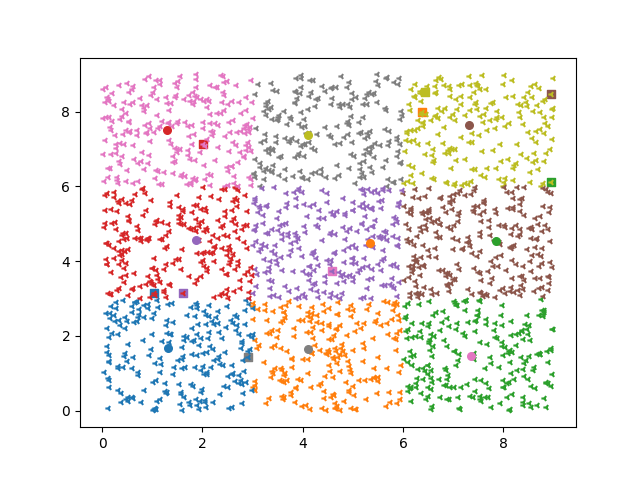
\includegraphics[height=7cm]{Figure_1.png}
        \caption{样本点数量为$2000$,欧氏距离度量,圆点是计算的聚类中心}
    \end{minipage}
 \end{figure}
 改变度量方式为曼哈顿距离
 \begin{figure}[H]
    \centering
    \begin{minipage}[t]{1.0\linewidth}
        \centering
        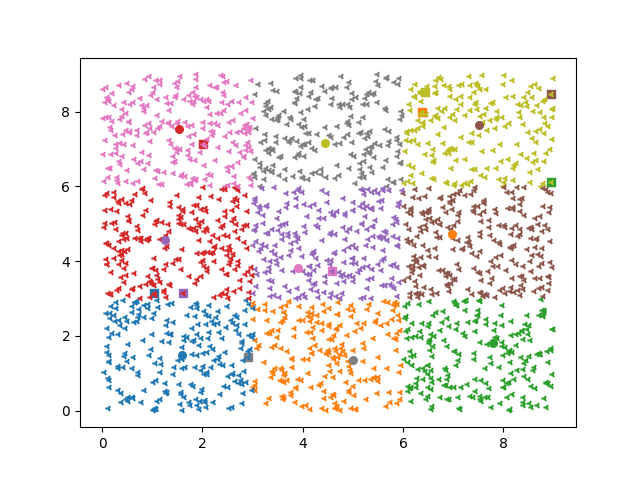
\includegraphics[height=7cm]{Figure_2.png}
        \caption{样本点数量为$2000$,曼哈顿距离度量}
    \end{minipage}
 \end{figure}
再次修改度量方式为切比雪夫距离
\begin{figure}[H]
    \centering
    \begin{minipage}[t]{1.0\linewidth}
        \centering
        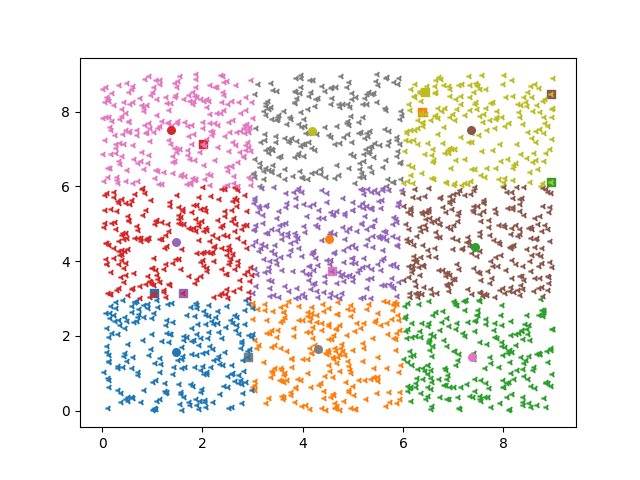
\includegraphics[height=7cm]{Figure_3.png}
        \caption{样本点数量为$2000$,切比雪夫距离度量}
    \end{minipage}
 \end{figure}
 可以看大度量方式不同,最后聚类出来的结果也会不同。事实上三种不同的度量方式各有特点
 $l1$距离计算的是向量中各个维度之间的差的绝对值的和,即所有差值的绝对值之和。等距线是方形,适用于特征在数据中不是呈正态分布的情况下,譬如本次实验使用的均匀分布就适用这种情况。
$l2$距离则是计算向量中各个维度之间的差的平方和的平方根,即差值的平方和的开方。其等距线是圆形,特别适合具有一定中心趋势的样本分布,比如正态分布。
$l\infty$距离计算的是向量中各个维度之间差的绝对值的最大值。适用于选择距离绝对差异最大的特征。

从结果上来看,切比雪夫距离实现的聚类结果更加均匀,不过曼哈顿距离在整个计算过程中,移动的幅度是三者中最小的,这可能与数据均匀分布的位置有关系,曼哈顿距离度量在这种条件下更容易找到一个相对稳定的聚类结果。
\end{document}